\newcommand{\Treebeard}{{\sc {Treebeard}}}
\newcommand{\op}[1]{{\texttt {#1}}}

\section{Compiler Overview}
Figure \ref{Fig:CompilerStructure} shows the high level structure of \Treebeard. 
The input to \Treebeard{} is a JSON serialized decision forest model, it supports popular frameworks like XGBoost and LightGBM and is extensible to other frameworks.
Given an input model our compiler generates optimized inference code. Specifically it generates a callable batch inference function \op{predictForest} that given an array of inputs, outputs an array of model predictions. 
 
\Treebeard{} specializes the code generated for inference by progressively optimizing and lowering a high level representation of the \op{predictForest} function down to LLVM IR \cite{LLVM}.
%Treebeard first constructs a high level representation of the decision forest inference operation. 
At the highest level (HIR) optimizations like tree tiling and ordering are applied to compact and balance the trees and group structurally identical trees in the forest so that they can share the same code. It then lowers to a mid-level IR (MIR) where loop optimizations like loop unrolling and parallelization are applied. At the lowest level of IR \Treebeard{} applies layout optimizations and generates vectorized code to take advantage of SIMD instructions where applicable. 
LLVM is then used to JIT compile the generated IR to executable code. The following sections describe each level of the IR and their lowering in more detail.

 %The specified set of options includes information such as the batch size, the type of the input features, the type for node thresholds and the type for feature indices \TODO{There are also several optimization related inputs like tile size, type of tiling, pipeline depth etc. Should we mention those?}. 


\begin{figure}
  \centering
  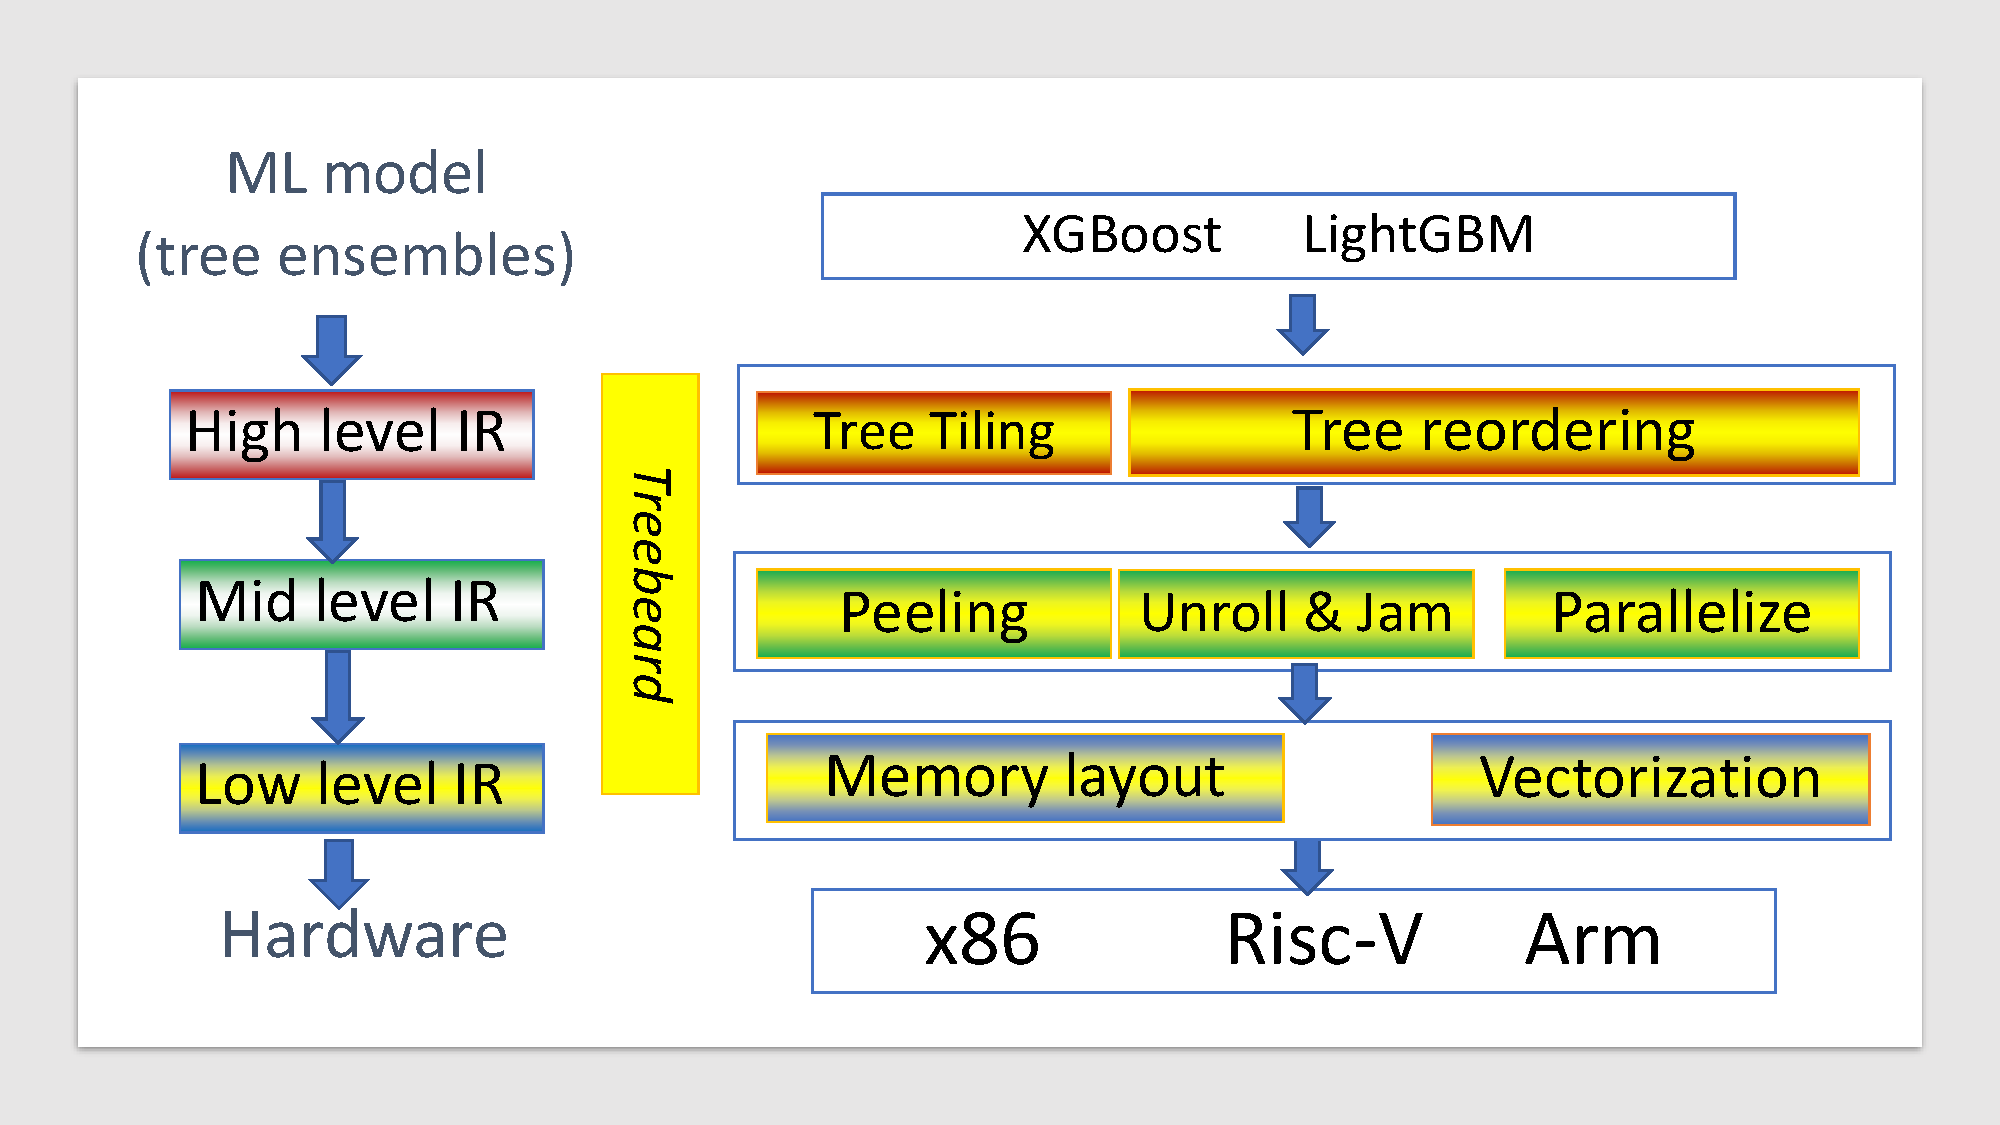
\includegraphics[width=\linewidth]{figures/compiler.pdf}
  \caption{Treebeard Compiler Structure}
  \label{Fig:CompilerStructure}
\end{figure}

%\TODO{Should we describe the dialect's type system?}
\TODO{Kr : consider focusing on the example instead of verbose description of optimizations. This section can be short, descriptions can come in later sections.}
\subsection{High Level IR}
As a first step \Treebeard{} parses the input and generates a single MLIR operation, \op{predictForest} that represents inference using the input model on a set of rows. 
At this level the operator simply contains a collection of binary trees. Two optimizations, tiling and tree ordering are applied at this level. The objective of tiling is to group nodes together so that the tree can be walked one tile at a time instead of one node at a time. We demonstrate that tiling can specialize the traversal of individual trees to either balance heavily skewed trees or proritize walks leading to higher probability leafs. Figure~\ref{ttile} shows examples of the tiling transformation. \TODO{kr: draw and explain example}. 

The objective of tree padding and ordering is to group identically structured trees so that they can share the same traversal code. The \op{predictForest} function is now lowered to MIR with separate loop nests generated for traversing a group of identical trees. The generated MIR code is as shown below. 
\TODO{show unoptimized loop nest as a listing}.


%The operation contains within it a tree based representation of the model that can be manipulated by optimizing transformations. Transformations on the model such as tiling, tree reordering and leaf padding are done at this level. The structure of the loop nest to walk the iteration space of trees and inputs is also decided at this level of the IR. \TODO{Should we mention that there is a scheduling language to decide this?}

\begin{lstlisting}[language=C++]
func Predict(float rows[batchSize]) {
  predictions = predictForest(rows) 
  return rows
}
\end{lstlisting}

\subsection{Mid Level IR}
The Mid Level IR optimizes the loop structures and tree walks. The order in which the iteration space of trees and inputs is walked is determined and loop nest are re-ordered if necessary. Loop peeling makes use of tree specific information about the levels at which leafs start to occur, to split the traversal loop into two parts, one that traverses the tree a constant number of steps (say upto first leaf) and an eplilogue that traverses the rest. Unroll and Jam, unrolls the inner loop and interleaves traversal steps so that a single tree is simultaneously traversed by multiple inputs. Usually when applied after peeling, it unrolls the first split almost entirely. \TODO{add figure with example, and text where appropriate above}. Finally, the outermost loop is parallelized by leveraging existing MLIR passes.
The \op{predictForest} function is now lowered to LIR with placeholder operators \op{isLeaf}, \op{traverseTile}, \op{getLeafValue} as shown below.  

\subsection{Low Level IR}
Optimizations at the LIR specialize the implementation of placeholder operators to the specific hardware. 
 For example, \op{traverseTile} is lowered into a series of operations to load thresholds, feature indices and features, compare the features with the thresholds and compute the next node to evaluate. Low level ISA instructions are picked (instruction selection) to implement these functions efficiently, for example vector instructions are introduced to exploit SIMD capabilities of the underlying hardware. This stage also determines the memory layout of the trees, the goal of the layout optimizations is to enable the traversal of the tree and implement checks like \op{isLeaf} at low memory overhead. 
\TODO{example}This IR is then lowered directly to LLVM IR and JITted.\\
\\
  \noindent
Note that all the optimization described so far are orthogonal and can be applied independent of each other. However, as we will see in detail over the next few sections, they do compliment each other. Padding and tree tiling discussed before help balance the tree, tiling in addition reduces the depth of the tree. These help peeling and unrolling eliminate most of the branches and loop checks in the innermost loop, producing mostly simple straightline code. This code is usually amenable to low level optimizations like vectorization.  



\begin{lstlisting}[style=c++]
  // Constant that represents the model being compiled
  forest = ensemble(...)
  for i = 0 to 2 step 1 {
    prediction = 0
    for t = 0 to 4 step 1 {
      tree = getTree(forest, t) 
      node = getRoot(tree)
      while (isLeaf(tree, n)==false)  do {
        node = traverseTreeTile(tree, node, rows[i])
      }
      treePrediction = getLeafValue(tree, node)
      prediction = prediction + treePrediction
    }
    predictions[i] = prediction
  }
\end{lstlisting}

The IR listed above is a simplification of the actual IR. The actual IR is strongly typed and in SSA form.


